\section{Medidas de Dispersión Relativa}
Se utilizan para comparar dos o mas distribuciones en torno a la media.
\subsection{Coeficiente de Variación $(C_v)$}
Es una medida de dispersión relativa muy útil cuando:
\begin{itemize}
\item Los datos están en unidades diferentes.
\item Los datos están en las mismas unidades, pero las medias muy distantes.
\end{itemize}
\subsubsection{Cálculo del Coeficiente de Variación}
$$C_v=\dfrac{S}{\overline{x}} \hspace{1cm}\vee\hspace{1cm}  C_v=\dfrac{S}{\overline{x}}100\hspace{1cm}\textrm{Tanto Porciento} $$
\subsection{Momentos}
Son de uso frecuente los promedios de las series de potencias de las variables estos promedios reciben el nombre de \textit{Momentos.} Pueden definirse respecto a cualquier punto:
\begin{itemize}
\item Momentos Respecto a un punto
\item Momentos Respecto del Origen
\item Momentos Respecto a la Media o Momentos Centrales
\end{itemize}
\subsubsection{Momentos Respecto a un Punto $(M_{r,A})$}
\begin{multicols}{2}
\textbf{Datos Originales} 
\begin{center}
$M_{r,A}=\dfrac{\displaystyle\sum_{i=1}^{n}(x_i-A)^r}{n}$
\end{center}
\columnbreak
\textbf{Datos Agrupados}
$$M_{r,A}=\dfrac{\displaystyle\sum_{i=1}^{n}(y_i-A)^r\cdot f_i}{n}$$
\end{multicols}
\subsubsection{Momentos Respecto del Origen $(M_r')$}
\begin{multicols}{2}
\textbf{Datos Originales} 
\begin{center}
$M_{r,A}=\dfrac{\displaystyle\sum_{i=1}^{n}(x_i)^r}{n}$
\end{center}
\columnbreak
\textbf{Datos Agrupados}
$$M_{r,A}=\dfrac{\displaystyle\sum_{i=1}^{n}(y_i)^r\cdot f_i}{n}$$
\end{multicols}
\subsubsection{Momentos Respecto a la Media $(M_r)$}
\begin{multicols}{2}
\textbf{Datos Originales} 
\begin{center}
$M_{r}=\dfrac{\displaystyle\sum_{i=1}^{n}(x_i-\overline{x})^r}{n}$
\end{center}
\columnbreak
\textbf{Datos Agrupados}
$$M_{r}=\dfrac{\displaystyle\sum_{i=1}^{n}(y_i-\overline{y})^r\cdot f_i}{n}$$
\end{multicols}
\section{Medidas de Forma}
\subsection{Coeficientes de Asimetría}
\begin{itemize}
\item Primer Coeficiente de Pearson $(S_p)$
$$S_p=\dfrac{\overline{x}-M_0}{S} \hspace{1cm} \textrm{en distribuciones Unimodales}$$
\item Segundo Coeficiente de Pearson $(S_p)$
$$S_p=\dfrac{3(\overline{x}-M_e)}{S}$$
\end{itemize}
\section{Medidas de Concentración}
Las medidas de concentración sirven para estimar el grado de igualdad en el reparto o grado de desigualdad de la distribución de cantidades económicas, riquezas, sueldos, etc. También sirve para analizar la concentración poblacional de un terriorio.
\subsection{Indice de Gini $(G)$}
Mide el grado de concentración a través de la diferencia entre $p_i$ y $q_i$ correspondientes, donde $p_i$ y $q_i$ son porcentajes acumulados de la distribución.\\${ }$\\La sumatoria es desde $i=1$ a $k-1$ porque resultaría en cero.
\subsubsection{Cálculo}
$$G=\dfrac{\displaystyle\sum_{i=1}^{k-1}(p_i-q_i)}{\displaystyle\sum_{i=1}^{k-1}p_i}$$
Observar que $0\leq G \leq 1$ y $0\leq\frac{G}{2}\leq \frac{1}{2}$.
\subsubsection{Interpretación de $\frac{G}{2}$}
Si $\frac{G}{2}>10\%$ se considera que la distribución es alta.
\subsection{Curva de Lorenz}
\begin{center}
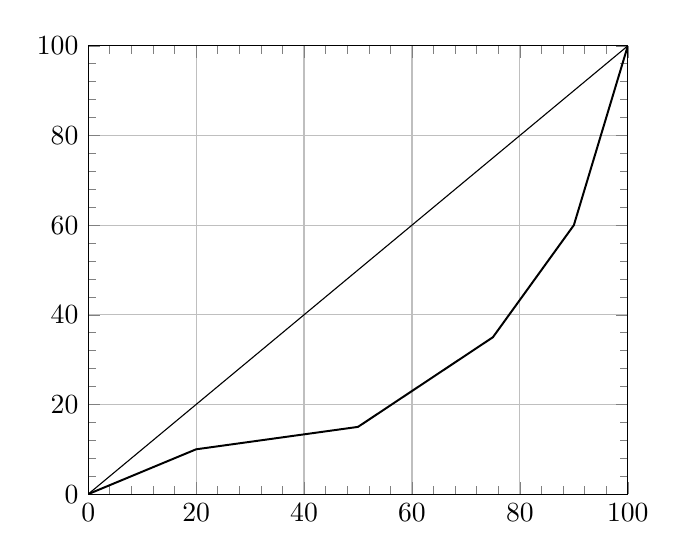
\begin{tikzpicture}
\begin{axis}[
    xmin=0, xmax=100,
    ymin=0, ymax=100,
    minor tick num = 4,
    grid,
    ]
\addplot[color=black,line width=0.25mm] plot 
    coordinates { (0,0) (20,10) (50,15) (75,35) (90,60) (100,100)};
\addplot[color=black] plot
    coordinates { (0,0) (100,100)};
\end{axis}
\end{tikzpicture}
\end{center}